\section{Building the Engine}

In this section we detail all the work that has been done on building our model which is the backbone of our engine. We start by describing the intuition behind using Natural Language Processing, then introduce N-gram models as our NLP technique of choice and close by describing how we incorporated that into our completion engine.

\subsection{Token Analysis}
Prior research in computer networking hints that we should expect network configurations to share a common set of stanzas and thus implicitly tokens~\cite{Benson}. As Hindle,\textit{et al.} 2012~\cite{naturalness} pointed out, regularities in bodies of texts can be easily exploited by NLP techniques. We hope to find and use such regularities in network configurations to generate suggestions.\\

In~\cite{complexity} researchers identified a few key design decisions commonly made by network operators. Network configurations are designed to be homogeneous as a means of easy maintenance, where some operators start off with common configuration templates with varying parameters. They may then tweak these templates to achieve specialized routing roles if needed. Thus one can posit that configurations across devices in a given network may share a lot of the same tokens, subnets and sometimes even complete stanzas (such as Access Control Lists). To confirm our hypothesis, we took configurations from a large university (University A as described in Section 4) network and split up each configuration file into a list of tokens. Tokens included all keywords and subnets with punctuation and newline characters stripped off. For every file we then plotted the percentage of tokens and statements that exist in other router configuration files.\\

Our results show that most of each file could be rebuilt from existing statements in routing configurations due to the amount of tokens they share. The statement similarity is particularly interesting as it shows that some of these router configurations had a large percentage of complete statements that they shared with the rest of the network. Given our results, and the observations made by~\cite{complexity} about how networks are configured, we can confidently hypothesize that most token suggestions can be generated from analyzing other existing configurations. This effectively makes all router configuration histories a part of the search space for our NLP model. 

\begin{figure}[H]
	\centering
	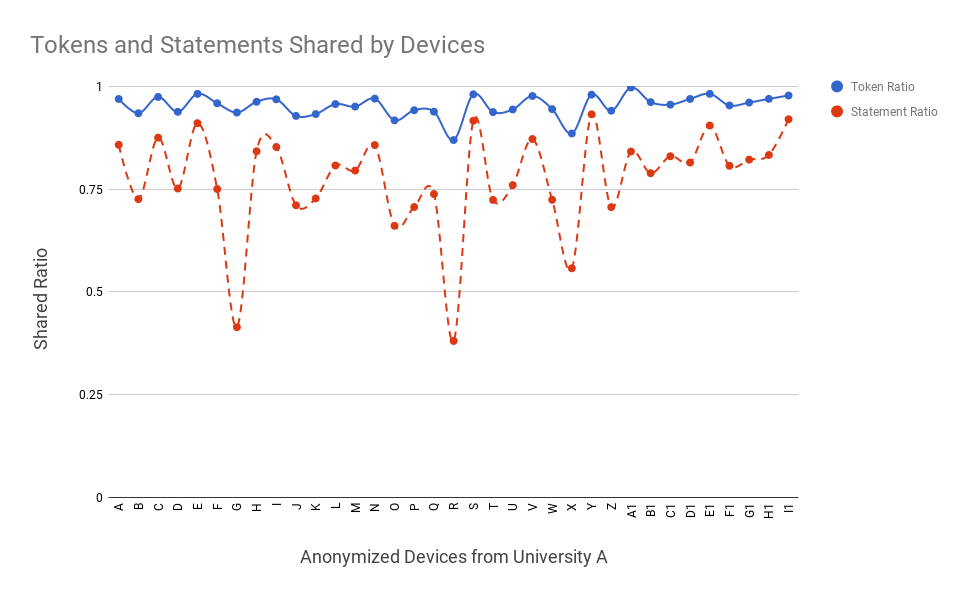
\includegraphics[width=\textwidth]{chart.png}
	\caption{The plot shows how many tokens and statements a router configuration holds in common with the rest of the network. The data was taken from a large research university.}
\end{figure}

\subsection{N-gram Models}

Given that token regularities existed in network configurations, we employ NLP techniques to make use of token histories. As mentioned in Section 2.2, we use N-gram models as a basis of our engine. Here we briefly describe the theory behind these models. Consider a sequence of tokens in a body of text (in our case, network configurations). We can statistically model how likely tokens are to follow other tokens. We accomplish this by calculating the conditional probabilities of certain tokens appearing in the text. Given a sequence of tokens $a_1,a_2,a_3,...,a_n$, we can calculate the probability of $a_2$ occurring given that $a_1$ has already occurred i-e $p(a_2 | a_1)$. We continue by calculating the probability of $a_3$ given $a_2$, and so on. Since we looked at two tokens at a time, this is called a bigram model. More generally, predicting how likely a token is to show up based on the previous $n-1$ tokens is called an N-gram model. In our work, we used bigram and trigram models. Any higher number of N-grams would have required a larger data set to train.\\

The probabilities for suggesting a token pair are estimated by using some scoring function. Often a function may simply count the frequency by which a given pair occurs in the training data and calculate the probability as a ratio of frequency of the pair to the total token count. However, we utilize likelihood estimators as they provided good accuracies for Hindle,\textit{et al.} and have been known to work well for N-gram models~\cite{manning}. Likelihood estimators have an added advantage of generally being more appropriate for sparse data than other tests. Our system internally uses the Manning and Schutze (5.3.4) version of likelihood estimators~\cite{manning}.

One problem that often emerges in N-grams is that high frequency and low variance can be accidental. If the two constituent words of a frequent. For example, some bigrams like ``ip address'' may show up together just because  are frequently ``ip'' and ``address'' are highly occurring words in of themselves even if they do not form a collocation. Researchers will thus use various forms of hypothesis testing to obtain values that better inform the model whether word pairs occur together more often than chance. We chose likelihood ratios as our hypothesis tests of choice. The two hypotheses for a bigram $w_1w_2$ in our case would be:

\begin{center}
Hypothesis 1 ($H_1$): $P(w_2|w_1) = p = P(w_2|\neg w_1)$ \\
Hypothesis 2 ($H_2$): $P(w_2|w_1) = p_1 \neq p_2 = P(w_2|\neg w_1)$	\\	
\end{center}

Hypothesis 1 is a formalization of independence (the occurrence of $w_2$ is independent of the previous occurrence of $w_1$). Hypothesis 2 informs us of the dependence between the words which is good evidence for an interesting collocation. Assuming a binomial distribution ($b(k; n,x)$), the likelihood functions are as follows:

\begin{center}
$L(H_1) = b(c_{12}; c_1,p) b(c_2)-c_{12}; N-c_1,p)$\\
$L(H_2) = b(c_{12}; c_1,p_1) b(c_2)-c_{12}; N-c_1,p_2)$
\end{center}

Here, we use maximum likelihood estimates for $p,p_1$ and $p_2$ with $c_1,c_2,c_{12}$ representing the counts for $w_1,w_2$ and $w_1w_2$ respectively, and $N$ being the sample size:end
\begin{center}
$p=\frac{c_2}{N}$\\
$p_1=\frac{c_{12}}{c_1}$\\
$p_2=\frac{c_2-c_{12}}{N-c_1}$
\end{center}

A likelihood ratio would thus be the ratio of $L(H_1)$ and $L(H_2)$.

\subsection{Placeholders}
We next add a networking specific optimization by incorporating some preprocessing steps to substitute certain parameters with generic tokens. For example, since IP addresses and subnets tend to vary a lot and add noise to the data, we replaced them with placeholders. Having these generic tokens in lieu of parameters helps the engine suggest places where parameters may be entered without trying to predict exact values, which is extremely difficult given our pure NLP approach. In Section 6, we consider other approaches to help suggest parameters such as IP addresses. In Section 5, we also look at the effect of every individual placeholder on the accuracies. We should also note that our initial analysis showed that the engine was trying to predict what the user would enter after a complete configuration statement. We observed that there was little correlation between the end token of a line and the starting token of the next line. We thus altered our model to only suggest tokens that appear on the same line.\\

\subsection{Implementation}

N-gram models provided us with a strong foundation on which we could build a specialized completion engine. We developed a program in Python which reads in configuration files and builds a trigram model, using the NLTK package~\cite{nltk}. NLTK also allows us to easily incorporate likelihood ratios as a means of scoring the N-grams. We wrote additional scripts to perform analyses and generate graphs. For our analyses, all individual tests were run in parallel to cut down on runtime. Our scripts were run on a 22-Core Intel(R) Xeon(R) CPU E5-2640 v4 @ 2.40GHz server with 128 GB of RAM running Ubuntu 16.04.4 LTS.\\ 



